\documentclass[acmtog]{acmart}
\usepackage{graphicx}
\usepackage{subfigure}
\usepackage{natbib}
\usepackage{listings}
\usepackage{bm}
\usepackage{amsmath}

\definecolor{blve}{rgb}{0.3372549 , 0.61176471, 0.83921569}
\definecolor{gr33n}{rgb}{0.29019608, 0.7372549, 0.64705882}
\makeatletter
\lst@InstallKeywords k{class}{classstyle}\slshape{classstyle}{}ld
\makeatother
\lstset{language=C++,
	basicstyle=\ttfamily,
	keywordstyle=\radiance{blve}\ttfamily,
	stringstyle=\radiance{red}\ttfamily,
	commentstyle=\radiance{magenta}\ttfamily,
	morecomment=[l][\radiance{magenta}]{\#},
	classstyle = \bfseries\radiance{gr33n},
	tabsize=2
}
\lstset{basicstyle=\ttfamily}

% Title portion
\title{Assignment 4: {Global Illumination}}

\author{Name:\quad Tian Haoyuan  \\ student number:\ 2020533013
\\email:\quad tianhy@shanghaitech.edu.cn}

% Document starts
\begin{document}
\maketitle

\vspace*{2 ex}

\section{Introduction}
Works that have been done are as follows.
\begin{itemize}
	\item Task1 Path tracing with Monte Carlo integration
	\item Task2 Ideal diffuse BRDF and area light source
	\item Task3 Acceleration structure: BVH
	\item Bonus1 The ideal specular or glossy specular BRDF
	\item Bonus2 The translucent BRDF with refraction
	\item Bonus3 Advanced BVH with higher performance
\end{itemize}

\section{Implementation Details}
\subsection{Path tracing with Monte Carlo integration}
This task is related with integrator.cpp, specifically function render(), radiance, and directLighting() as well.
The task of render() function is to set every pixel on the target image, and for each pixel, we would like to do \#spp times of sampling within the pixel to evaluate it.
The role of radiance() function is to get the radiance of a single sampling (one single ray generated from camera).\\
The radiance at the ray-intersected interaction should be composed of direct lighting and indirect light (limited by max\_depth).
Naturally if the interaction type is light, then it should just be the emission of the light; otherwise it should be geometry type, we should add up its direct and indirect lighting of deffusion on brdf, which will be implemented in task 2.
As for direct lighting, we should generate a ray from interaction position to the light, see whether it would be blocked by some obstacles, and finally compute the lighting again by brdf.\\
Then goes the indirect lighting, we should add up $L*fr*cos(\theta)/pdf$ iteratively. So I update beta after making direct lighting, and multiply the direct lighting of next depth then add it up.

\subsection{Ideal diffuse BRDF and area light source}
This task is related with bsdf.cpp, to complete the whole render process. So after we go through this task, we should have a simple template to do global illumination.\\
We use cosine weighted to construct ideal diffusion, leading to the formular that the pdf should be $p(w)=c*cos(\theta)$, where $\theta$ is uniformally distributed in range $[0,2\pi]$. The integration of the pdf shoud satisfy $$\int_{H^2}c*\cos{\theta}dw=1,$$
$$\int_{0}^{2\pi}\int_{0}^{\frac{\pi}{2}}c\cos{\theta}\sin{\theta}d\theta d\phi=1.$$
So $c=\frac{1}{\pi}$, and the pdf should be $$p(w)=c\cos{theta}=\frac{\cos{\theta}}{\pi}.$$\\
The period result is as follows:
\begin{figure}[h]
	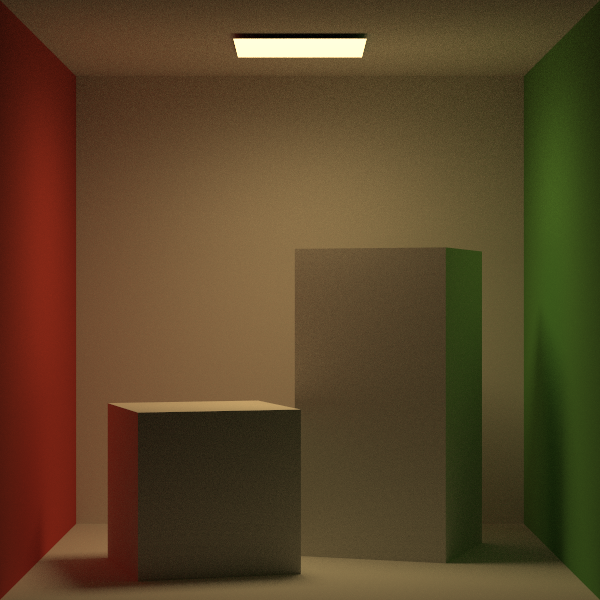
\includegraphics[width=6.0cm,height=6.0cm]{without_bvh.png}
	\caption{result before implementing bvh}
\end{figure}\\
The time cost of rendering this $600\times 600$ image is 173s.

\subsection{Acceleration structure: BVH}
I straightly construct BVH with SAH, so there is no rendering cost result for simple BVH, but SAH can naturally be considered as a naive BVH with a heuristic, so I would also like to explain the implementation detail of a naive BVH.\\
The major part is in geometry.cpp, the bvhbuild and bvhhit function, and I also alter the BVHNode structure, keeping the start index and the number of triangles instead of keeping the triangle vector.\\
The triangle intersection function are implemented just the same as that is in assignment3. Then comes the bvh building function, which is implemented iteratively. To construct simple bvh, we should always split the bounding box until it could be considered as a leaf node, and keep the splited bvh node as the children of the current node.
The simpliest method is to split along the longest axis, while SAH has some other heuristic that I will talk about later.\\
The bvh hit function should traverse down the tree until it is a leaf node, where we can do triangle intersection within the leaf nodes.

\subsection{Advanced BVH with higher performance}
Here I take SAH as an advanced BVH, the performance will be shown later.\\
The main idea is that, in simple BVH, there may happen that two child bvh nodes' bounding box can have a huge overlap from a particular split, leading to the consequence that the split is just so inefficient that the program may do bvh hit in similar box for multiple times.\\
To avoid this redundant cost, I would like to minimize some cost when I do split on a single bounding box. For every internal node, the cost I take is
$$COST = P(A)*N(A) + P(B)*N(B),$$
where $P(A)$ is the probablity that the ray that hit the bounding box of current node would also hit the bounding box of A, which can be estimated by the superficial area of the bounding boxes, and $N(A)$ is the number of triangles within the bounding box of A. I traverse to minimize the cost and do split after that, the performance is better than naive BVH.
The result is as follows,
\begin{figure}[h]
	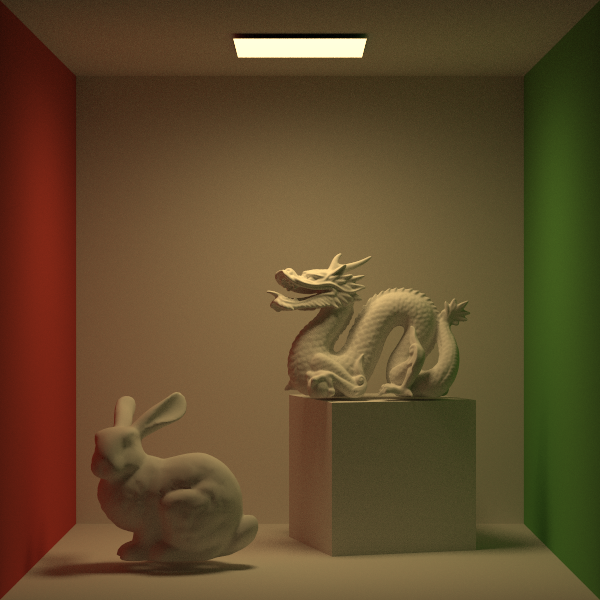
\includegraphics[width=6.0cm,height=6.0cm]{bvh_large.png}
	\caption{result with sah bvh}
\end{figure}\\
The picture is rendered in 153s, comparing to the difference that shown on course page: simple bvh large mesh (125s) to simple mesh (110s), that we can see the bvh and advanced bvh(SAH) should be correctly implemented.

\subsection{The ideal specular or glossy specular BRDF}
To implement ideal specular,
I would like to add a IdealSpecular class inheriting BSDF,
that highly resembles IdealDiffusion. Thisishould be ideal reflection, so the return value of evaluate should be the origin color of the material, and the pdf should be 1.\\
The result is as follows,
\begin{figure}[h]
	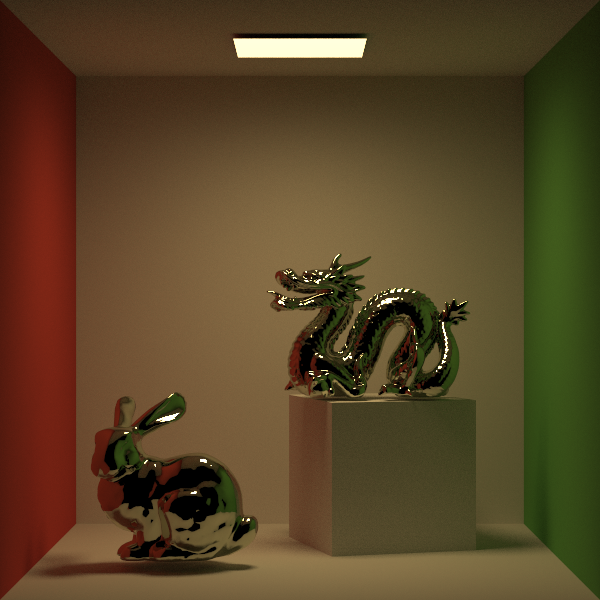
\includegraphics[width=6.0cm,height=6.0cm]{specular.png}
	\caption{ideal specular}
\end{figure}\\
\subsection{The translucent BRDF with refraction}
As is implemented in the last part, we should also add a class Translucent in bsdf.h that inherits BSDF, and we have to overwrite its pdf, evaluate function and so on. *Reference: https://www.pbr-book.org/3ed-2018/Reflection\_Models/Specular\_Reflection\_and\_Transmission.
Get ready with Fresnel reflectance first, that is $$F_r = \frac{1}{2}(r_{\parallel}^2+r_{\perp}),$$
where $$r_{\parallel}=\frac{\eta_t\cos\theta_i-\eta_i\cos\theta_t}{\eta_t\cos\theta_i+\eta_i\cos\theta_t},$$
$$r_{\perp}=\frac{\eta_i\cos\theta_i-\eta_t\cos\theta_t}{\eta_i\cos\theta_i+\eta_t\cos\theta_t}.$$
And in refract(), if $$1-\cos^2{\theta_t}=\frac{\eta_i^2}{\eta_t^2}sin^2{\theta_i}>1,$$
namely there does not exist real $\theta_t$ to satisfy $\cos{\theta_t}=\sqrt{1-\frac{\eta_i^2}{\eta_t^2}sin^2{\theta_i}},$ we should say that there is no refraction at this position, and consider its reflection; otherwise, compute its refraction direction wo.\\
While evaluating, check to switch $\eta_i$ and $\eta_t$ since the ray may come from the inner part of the object or from outside.\\
The result is as follows,
\begin{figure}[h]
	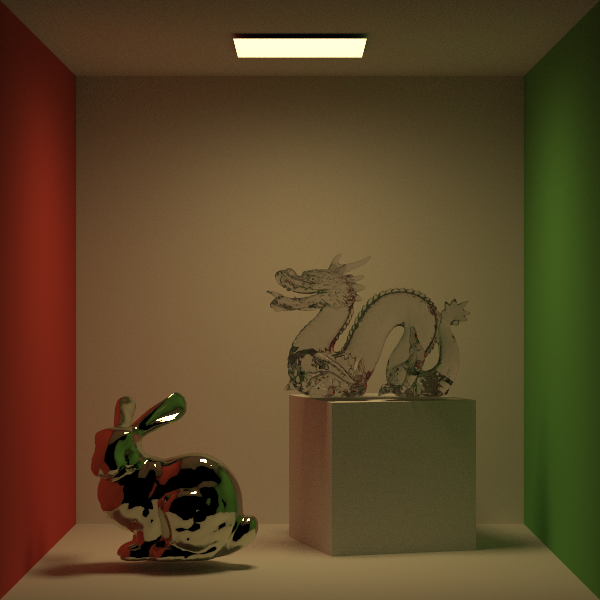
\includegraphics[width=6.0cm,height=6.0cm]{translucent.png}
	\caption{translucent}
\end{figure}\\
\section{Results}
% pictures should be in
* For coherence of expression I put the bonus advanced BVH next to must part simple BVH in this report.
\end{document}
